\documentclass[11pt,letterpaper]{article}
\usepackage[T1]{fontenc}
\usepackage[utf8]{inputenc}
\usepackage{lmodern,amsmath,amssymb,amsthm,mathtools}
\usepackage[margin=1in,headheight=15pt]{geometry}
\usepackage{microtype,booktabs,longtable,tabularx,array,enumitem}
\usepackage{xcolor,hyperref,fancyhdr,tikz,listings}
\usetikzlibrary{arrows.meta,positioning}
\definecolor{navy}{HTML}{18334D}
\definecolor{teal}{HTML}{087F83}
\definecolor{pale}{HTML}{EDF4F6}
\hypersetup{colorlinks=true,linkcolor=navy,citecolor=teal,urlcolor=teal,
 pdftitle={Beyond Dirichlet GRH: audit and transfer analysis},
 pdfauthor={Research analysis prepared for Vladimir Reshetnikov}}
\urlstyle{same}
\pagestyle{fancy}
\fancyhf{}
\fancyhead[L]{\small\textsc{Beyond Dirichlet GRH}}
\fancyhead[R]{\small Source audit and transfer analysis}
\fancyfoot[C]{\thepage}
\setlength{\parskip}{5pt}
\setlength{\parindent}{0pt}
\setlist{itemsep=3pt,topsep=5pt}
\setcounter{tocdepth}{2}
\newtheorem{theorem}{Theorem}[section]
\newtheorem{proposition}[theorem]{Proposition}
\newtheorem{corollary}[theorem]{Corollary}
\newtheorem{lemma}[theorem]{Lemma}
\theoremstyle{definition}
\newtheorem{definition}[theorem]{Definition}
\theoremstyle{remark}
\newtheorem{remark}[theorem]{Remark}
\newcommand{\Q}{\mathbb Q}
\newcommand{\Z}{\mathbb Z}
\newcommand{\C}{\mathbb C}
\newcommand{\R}{\mathbb R}
\newcommand{\N}{\mathbb N}
\newcommand{\eps}{\varepsilon}
\newcommand{\Rea}{\operatorname{Re}}
\newcommand{\Ima}{\operatorname{Im}}
\newcommand{\ord}{\operatorname{ord}}
\newcommand{\tr}{\operatorname{tr}}
\newcommand{\Gal}{\operatorname{Gal}}
\newcommand{\Cl}{\operatorname{Cl}}
\newcommand{\Sha}{\operatorname{Sha}}
\newcommand{\ind}{\mathbf 1}
\newcommand{\code}[1]{\texttt{\small\detokenize{#1}}}
\newcommand{\src}[1]{\par{\small\color{navy}Source: \nolinkurl{grh/src/#1}}\par}
\newcommand{\status}[1]{\textbf{\color{teal}#1}}
\newcolumntype{Y}{>{\raggedright\arraybackslash}X}
\lstset{basicstyle=\ttfamily\small,breaklines=true,columns=fullflexible,
 keepspaces=true,frame=single,rulecolor=\color{pale},showstringspaces=false}
\begin{document}
\begin{titlepage}
\thispagestyle{empty}
{\color{teal}\large RESEARCH REPORT}\par
\vspace{0.7in}
{\color{navy}\Huge\bfseries Beyond Dirichlet GRH\par}
\vspace{0.25in}
{\LARGE A source audit and a research transfer map\par}
\vspace{0.15in}
{\Large for \texttt{lsernau/grh-lean}\par}
\vspace{0.5in}
{\large Prepared for Vladimir Reshetnikov\par}
{\large November 25, 2026 (Pacific date)\par}
\vspace{0.35in}
\begin{tabularx}{\textwidth}{@{}lY@{}}
\toprule
Repository & \url{https://github.com/lsernau/grh-lean}\\
Audited commit & \code{72fead102f663d5c7a407964a13dc0cf9d977207}\\
Lean & \code{leanprover/lean4:v4.35.0}\\
Mathlib & \code{56a005855ea17e0b0958f73ec801ae140b0a1679}\\
\bottomrule
\end{tabularx}
\vspace{0.35in}
\colorbox{pale}{\begin{minipage}{0.94\textwidth}
\vspace{8pt}
\textbf{Finding.} There are concrete mathematical transfers: established
GRH-conditional classifications and bounds, a reusable determinant argument,
and a precise route toward a first nonabelian example. The source does not
already contain a general proof of Hecke or Artin GRH, Vandiver's conjecture,
or the Birch--Swinnerton-Dyer conjecture.

\textbf{Evidence.} We inspected the pinned source and reproduced static and
finite arithmetic checks. Independent build and kernel checks are reported by
the authors and external verification projects. We did not rerun the full Lean
development. The new Lean examples are explicitly uncompiled.
\vspace{8pt}
\end{minipage}}
\vfill
This report separates consequences of the exported theorem, independently
proved reductions, exact finite calculations, and research obligations that
remain open. No priority claim is made for the extracted reductions.
\end{titlepage}

\begin{abstract}
We analyze the mathematics and formal interfaces of the shortened Lean
development of the Riemann hypothesis and Dirichlet GRH. The exported
statements genuinely use Mathlib's zeta and Dirichlet \(L\)-functions.
The distinctive mechanism combines short integral automorphic forms,
quantitative spanning, and a lower bound for twisted determinants. Their
common main term cancels, leaving a one-sided smoothed prime-sum bound.
Quadratic-twist separation and Landau's theorem convert that bound into zero
exclusion.

Immediate transfers include the value zero of the de Bruijn--Newman
constant and published norm-Euclidean field classifications. We prove a
general one-sided transform criterion and show that the source's
auxiliary-prime hypothesis can be weakened to a sufficiently populous
subfamily. We then formulate a fully explicit next target: the degree-two
Artin \(L\)-function associated with \(X^3-X-1\). Its positive tensor-square
coefficients admit the same analytic reduction, but two crucial arithmetic
and twist-selection inputs remain unproved. Finally, we identify a concrete
ramification obstruction to a naive K-theory transfer and distinguish
recent follow-on claims from theorems in this repository.
\end{abstract}
\tableofcontents
\clearpage

\section{Conclusions and their logical status}
\label{sec:conclusions}

\textbf{Yes, the repository can be used beyond its five exported statements.}
The cleanest immediate use is to supply a hypothesis in an existing theorem.
The most promising research use is to extract its arithmetic comparison
interfaces and rebuild them for a wider coefficient system. These are
different achievements and should be credited separately.

\begin{table}[ht]
\centering\small
\begin{tabularx}{\textwidth}{@{}p{0.27\textwidth}Yp{0.25\textwidth}@{}}
\toprule
Result or direction & What this report establishes & Status\\
\midrule
The exported RH and Dirichlet GRH & The statements, source pins, import
structure, and absence scan were inspected. & Source audit; external machine
checks reported.\\
\(\Lambda_{\rm DBN}=0\) & RH gives \(\Lambda_{\rm DBN}\le0\); Rodgers--Tao
give the reverse inequality. & Known implication, with GRH/RH input supplied.\\
Norm-Euclidean cyclic fields of degree \(5,7\) & The GRH assumptions in the
published classifications match Dirichlet GRH. & Published conditional
theorems can be discharged.\\
Sparse auxiliary-prime criterion & A large enough subset of valid witnesses
replaces a universal auxiliary-prime hypothesis. & Paper-level proof here;
no novelty or Lean-check claim.\\
\(S_3\) Artin \(L\)-function of conductor \(23\) & Exact positivity,
factorizations, and a conditional zero-exclusion theorem. & Two substantive
inputs remain missing.\\
Vandiver and integral K-groups & A precise failed hypothesis and a
pointwise-witness issue are identified. & No new vanishing theorem proved.\\
\bottomrule
\end{tabularx}
\caption{Reading the claims at the right strength. Consequences using the
repository inherit its foundational and statement-interpretation assumptions.}
\end{table}

The report does not claim to be the first to observe standard consequences of
RH or GRH. In particular, a problem historically described as open may already
have a new proof, a new claim, or a published GRH-conditional resolution.
We checked recent primary sources to avoid treating the cyclic cubic
norm-Euclidean classification, for example, as a new open target.

The two most useful follow-up projects are concrete. For a relatively short
formal project, package the one-sided criterion with the weaker
auxiliary-family condition of Section~\ref{sec:sparse}. For a substantial
mathematical project, work on the explicit degree-two target of
Section~\ref{sec:s3}, beginning with its missing arithmetic inequality.

\section{What the repository actually proves}
\label{sec:audit}

\subsection{Pinned source and endpoint statements}

The audited repository has the single commit
\code{72fead102f663d5c7a407964a13dc0cf9d977207}, authored November 25, 2026.
It supplies a readable edition \code{grh} and a compact edition
\code{grh-compact}. Both pin Lean \(4.35.0\) and the same Mathlib commit.
The mathematical work is attributed to Levent Alp\"oge with Claude; the
shortened version was produced by Luke Sernau, colleagues at Anthropic,
and Claude \cite{repo,announcement}.

The four auxiliary propositions in \code{src/Statements.lean} import only
Mathlib. The five theorems in \code{src/Main.lean} are:
\begin{enumerate}
\item \code{riemannHypothesis}: Mathlib's \code{RiemannHypothesis}.
\item \code{riemannZeta_eq_zero_re}: every zero of \(\zeta\), apart from the
negative even integers and the separately excluded point \(1\), has real
part \(1/2\).
\item \code{LFunction_ne_zero_of_half_lt_re}: for every positive modulus
\(N\), every Dirichlet character \(\chi\bmod N\), and every \(s\),
\[
 \Rea s>\tfrac12,\quad(\chi\ne1\ \text{or}\ s\ne1)
 \quad\Longrightarrow\quad L(s,\chi)\ne0.
\]
\item \code{LFunction_eq_zero_re}: every zero of any such \(L\)-function
in \(0<\Rea s<1\) lies on \(\Rea s=1/2\).
\item \code{LFunction_eq_zero_re_of_isPrimitive}: the same statement for
primitive characters, as a special case.
\end{enumerate}

The pole exception matters because an analytically continued meromorphic
object may be represented in Lean by a total function with a chosen value at
its pole. The theorems explicitly exclude the relevant point. They cover
imprimitive as well as primitive characters, but the Dirichlet zero-location
theorems make no assertion about zeros in \(\Rea s\le0\).

We inspected the pinned Mathlib definition of \code{RiemannHypothesis} and
the relevant zeta interface. There is no visible substitution of a different
endpoint function or an added GRH hypothesis. This is an interface check;
it is not an independent reconstruction of all analytic definitions or of
the entire formal proof.

\subsection{What was checked here, and what was reported elsewhere}

The bundled \code{code/static_audit.py} performs a nested-comment and
string-aware lexical scan, inventories every source file, records SHA-256
hashes, reads the build pins, and follows local imports. Its output is
\code{data/static_audit.json}.

\begin{center}
\begin{tabular}{@{}lrrr@{}}
\toprule
Edition & Lean source files & All source lines & Nonblank code lines\\
\midrule
Readable & 803 & 477,124 & 299,902\\
Compact & 794 & 112,827 & 76,149\\
\bottomrule
\end{tabular}
\end{center}

At module level, all 803 readable modules and all 794 compact modules are
reachable from \code{Main}. This says nothing about whether every declaration
inside a reachable module is needed by the final theorem. No local import
cycle or scanner warning was found. The working tree was clean.

The scan found no standalone occurrences in either \code{src} tree of
\code{sorry}, \code{admit}, \code{axiom}, \code{unsafe}, \code{opaque},
\code{native_decide}, \code{implemented_by}, \code{run_elab},
\code{run_cmd}, \code{elab}, \code{macro}, \code{initialize},
\code{ofReduceBool}, or \code{ofReduceNat}, after removing comments and
literals. This is a limited lexical check, not a parser or a replacement
for an axiom dependency audit.

Each edition also has a \code{Challenge.lean} containing intentional
\code{sorry} placeholders for Comparator. It lies outside \code{src},
is not imported by those source trees, and is not a default build target.
Treating those comparator placeholders as admitted steps in the main proof
would be a false alarm.

The README reports successful builds, the axiom set
\[
 \{\code{propext},\ \code{Classical.choice},\ \code{Quot.sound}\},
\]
and independent checker/Comparator acceptance. Sutherland's MIT verification
page reports checks of both editions at the same pinned commit
\cite{sutherland}. Rubinstein's compact verification page, in the version
read for this report, records 794 successful builds and 794 successful
module replays, with its further multi-kernel run still in progress
\cite{rubinstein}. These are attributed external reports. We did not
reproduce their large computations, and no full-build log from our own
execution is included.

This distinction supplies an accurate account of what this analysis adds
to the verification evidence.

\subsection{The scope of the term GRH}

The exported conclusion is \emph{Dirichlet GRH over \(\Q\)}. It is not the
statement that every Hecke, Artin, or automorphic \(L\)-function satisfies
GRH. Using high-rank unitary groups inside a proof does not enlarge the type
of its endpoint theorem.

The reading guide also warns that some internal background theories are
formulated in weaker, customized ways: certain Galois attachments are
approximate/dense-Frobenius statements, some local polynomials are
annihilating polynomials rather than characteristic polynomials, and a
general Weil--Deligne construction is not supplied. Such results may be
fully adequate for the proof. Their names alone do not justify importing
the strongest conventional theorem with a similar name.

\section{The mechanism worth transferring}
\label{sec:mechanism}

\subsection{The arithmetic bottleneck}

Fix a suitable modulus \(q\) and an odd auxiliary prime \(d\), and put
\[
 \lambda_{d,q}(n)=
 \ind_{n\equiv1\pmod q}\Lambda(n)\left(1-\left(\frac nd\right)\right).
\]
Here \(\Lambda\) is the von Mangoldt function and \((n/d)\) is the Legendre
symbol. The crucial remainder has the form
\begin{equation}\label{eq:remainder}
 R_{d,q}(x)=
 \sum_{n\le x}\lambda_{d,q}(n)\left(\frac1n-\frac1x\right)
 -\frac{\log x}{\varphi(q)}-c_{d,q}.
\end{equation}
The constant is chosen so that the smoothed error has the appropriate
normalization at infinity. Its exact analytic expression appears in
Section~\ref{sec:analytic}.

The source obtains an eventual \emph{upper} bound, not initially a
two-sided absolute-value estimate:
\[
 R_{d,q}(x)\le C_{q,\eps}x^{-1/2+\eps}.
\]
Obtaining this bound is where the large arithmetic construction is used.
The constant can be chosen independently of \(d\); the threshold beyond
which the estimate holds may depend on \(d\). No uniform threshold is
asserted here.

\begin{figure}[ht]
\centering
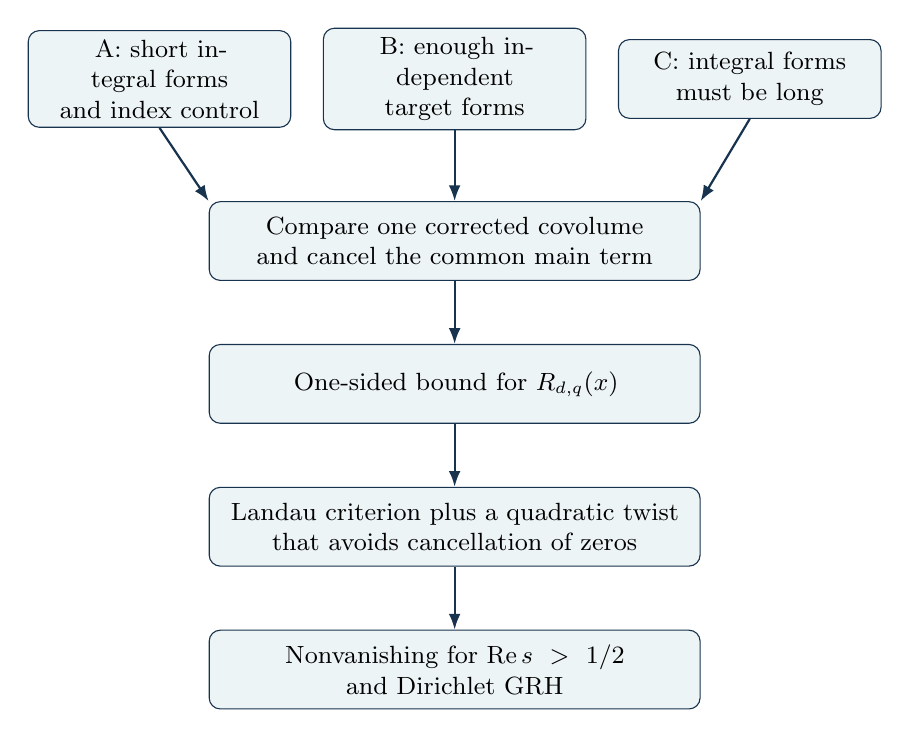
\begin{tikzpicture}[
 box/.style={draw=navy,rounded corners,fill=pale,align=center,
 font=\small,text width=3.1cm,minimum height=1cm},
 arrow/.style={-{Latex[length=2mm]},thick,draw=navy}]
 \node[box] (short) {A: short integral forms\\and index control};
 \node[box,right=4mm of short] (span) {B: enough independent\\target forms};
 \node[box,right=4mm of span] (long) {C: integral forms\\must be long};
 \node[box,below=9mm of span,text width=6cm] (cmp)
 {Compare one corrected covolume\\and cancel the common main term};
 \node[box,below=8mm of cmp,text width=6cm] (rem)
 {One-sided bound for \(R_{d,q}(x)\)};
 \node[box,below=8mm of rem,text width=6cm] (landau)
 {Landau criterion plus a quadratic twist\\that avoids cancellation of zeros};
 \node[box,below=8mm of landau,text width=6cm] (grh)
 {Nonvanishing for \(\Rea s>1/2\)\\and Dirichlet GRH};
 \draw[arrow] (short.south)--(cmp.north west);
 \draw[arrow] (span)--(cmp);
 \draw[arrow] (long.south)--(cmp.north east);
 \draw[arrow] (cmp)--(rem);
 \draw[arrow] (rem)--(landau);
 \draw[arrow] (landau)--(grh);
\end{tikzpicture}
\caption{The source's logical architecture. The last analytic step is
portable; the arithmetic construction that supplies its input is the
substantial barrier to a wider theorem.}
\end{figure}

The source constructs chains of theta lifts, meaning integral transforms
between spaces of automorphic forms, with chain length
\(m\asymp\sqrt{x}\). One direction controls the size and divisibility of
lifted forms. A second-moment calculation supplies enough independent
forms. A determinant argument supplies the opposing lower bound.

\subsection{Why the main terms cancel}

The following elementary comparison isolates the algebraic interface.

\begin{lemma}[Covolume comparison]\label{lem:comparison}
Let \(D\ge n>0\), \(n\ge\theta D\), \(0<\theta\le1\), \(m>0\), and
\(M,u,v,\delta\ge0\). Suppose some real \(V,\Delta,R\) satisfy
\[
 D(M-v)\le V+2\Delta,\qquad
 V\le n(M-mR+u),\qquad \Delta\le D\delta.
\]
Then
\begin{equation}\label{eq:comparison}
 mR\le u+\frac Dn(v+2\delta)
       -\left(\frac Dn-1\right)M
 \le\frac{u+v+2\delta}{\theta}.
\end{equation}
\end{lemma}
\begin{proof}
Combining the hypotheses gives
\[
 n\,mR\le n u+Dv+2D\delta-(D-n)M.
\]
Divide by \(n>0\), discard the last nonpositive term, and use
\(D/n\le1/\theta\) and \(u\le u/\theta\).
\end{proof}

In the actual proof, \(D\) is the target dimension, \(n\ge D/2\),
\(M\) is \code{mainAmount}, and \(R\) is \code{totalRemainder}. The final
arithmetic inequality is
\[
 m\,\mathrm{totalRemainder}\le f\,a\,(\log b)^5.
\]
After translating between cutoffs, the source gets
\[
 R_{d,q}(x)\le
 \frac{\varphi(q)(\log b)^6}{m}
 +|R_{d,q}(x_1)|+\log b\,|R_{d,1}(x_1)|.
\]
One chooses \(m\ge\sqrt{x}\), \(\log b\le2x^\eps\), and a much larger
\(x_1\) where existing prime-number-theorem estimates make the last two
terms small. In particular the source proves, at large integral \(x\),
\[
 R_{d,q}(x)\le(64\varphi(q)+3)x^{-1/2+6\eps}
 \quad(0<\eps<1/100).
\]
It then passes to real \(x\) and to the zero-free conclusion.
\src{New/Reduction/MainInequality.lean}
\src{New/Reduction/OneSidedBound.lean}

The square-root chain length explains the exponent. It does not license
replacing \(m\) by a larger value while holding all other estimates fixed.
The existence of the data, ranks, levels, sparse sets, denominator bounds,
and error budgets is tied to the parameter regime.

\subsection{A different favorable twist at each finite place}

One particularly useful interface is
\code{New.TwistedLattice.covolume_add_index_nonneg}.
For a partial basis \(y\), a complementary family \(z\) of size \(n'\),
and a family of injective lifts, it concludes
\begin{equation}\label{eq:twisted}
 0\le c+2\delta+n'(b_{\rm short}+b_{\rm denom})+b_{\rm volume}.
\end{equation}
Here \(c\) bounds a logarithmic squared covolume, \(\delta\) bounds the
index needed for integrality, and the remaining terms control the
complement and determinant ratios.

The important flexibility is that the favorable twist may be chosen
separately for each \(p\)-adic embedding. It need not be one twist that
works at every finite prime. However, the ratios comparing the twisted
determinants to the untwisted determinant must satisfy the source's
explicit height condition. This is how the local choices are made
compatible with a global product-formula argument.

To see the mechanism, write \(Z(\xi)\) for a lift determinant and
\(\Gamma(\xi)\) for the full Gram determinant of the lifted basis.
The proof factors \(\Gamma(1)\), at each allowed local twist \(\xi\), into
an integral term, a denominator term, and \(Z(1)/Z(\xi)\). The height
bounds add under multiplication. Archimedean norm bounds and the
nonvanishing of the full determinant then give \eqref{eq:twisted}.
Choosing independently good local objects without this comparison-height
control would not be justified.
\src{New/Reduction/Lattices/TwistedLattice.lean}

This interface is a strong candidate for reuse in other period, congruence,
and arithmetic-lattice arguments. Its applicability to any particular
new problem still requires constructing the maps, proving injectivity,
and supplying the integrality and height bounds.

\section{Concrete consequences available through published theorems}
\label{sec:consequences}

In this section the repository's exported theorem is used as the input.
The external theorems retain their original mathematical and computational
dependencies. We have checked the relevant statements and their scope;
we have not formalized their complete proofs.

\subsection{The de Bruijn--Newman constant is exactly zero}

For the usual heat deformation \(H_t\) of Riemann's \(\Xi\)-function,
the de Bruijn--Newman constant \(\Lambda_{\rm DBN}\) is characterized by
all zeros of \(H_t\) being real exactly when \(t\ge\Lambda_{\rm DBN}\).
RH is equivalent to \(\Lambda_{\rm DBN}\le0\). Rodgers and Tao proved
\(\Lambda_{\rm DBN}\ge0\) \cite{rodgers-tao}. Consequently,
\[
 \boxed{\Lambda_{\rm DBN}=0.}
\]
This is a precise answer to another longstanding exact-value question.
The deduction is a known composition of two theorems, not a new argument
about heat flow discovered in this analysis.

\subsection{Norm-Euclidean cyclic fields of degrees five and seven}

A number field \(K\) is norm-Euclidean when division with a smaller
remainder is possible using its absolute field norm:
for all \(\alpha,\beta\in\mathcal O_K\), \(\beta\ne0\), there exists
\(\gamma\in\mathcal O_K\) with
\[
 |N_{K/\Q}(\alpha-\gamma\beta)|<|N_{K/\Q}(\beta)|.
\]
Lezowski and McGown prove the following under GRH
\cite[Theorems 1.3 and 1.4]{lezowski-mcgown}.

\begin{center}
\begin{tabular}{@{}cl@{}}
\toprule
Degree of cyclic field & Exactly the norm-Euclidean discriminants\\
\midrule
\(5\) & \(11^4,\ 31^4,\ 41^4\)\\
\(7\) & \(29^6,\ 43^6\)\\
\bottomrule
\end{tabular}
\end{center}

They also establish nonexistence in the degrees
\[
 19,31,37,43,47,59,67,71,73,79,97.
\]
The GRH inputs concern the relevant Dirichlet characters (equivalently,
the abelian field zeta factorizations); these are within the repository's
scope. Thus the exported theorem discharges the GRH assumptions in these
published results. Their finite norm and exclusion calculations remain
part of the proofs and were not rerun here.

The corresponding cyclic \emph{cubic} classification is a poor novelty
target: an unconditional determination was already posted in 2025 and
revised in 2026 \cite{cyclic-cubic}. It may be reproved through GRH, but
should not be advertised as a newly settled question.

\subsection{Euler's sixty-five idoneal numbers}

One precise modern definition is that a positive integer \(n\) is
idoneal if the proper ideal class group of the quadratic order of
discriminant \(-4n\) has exponent dividing two. Equivalently, every
primitive positive definite form of that discriminant has an ambiguous
class. This is equivalent to the classical formulation connected with
prime tests using \(x^2+ny^2\); the equivalence is a theorem, not a
definition to be silently changed.

Weinberger's work, with the order-versus-field distinction clarified by
Kani, gives completeness of Euler's list under quadratic Dirichlet GRH
\cite{weinberger,kani,watkins}. The repository covers those characters,
so it supplies that hypothesis. The list is
\begin{align*}
&1,2,3,4,5,6,7,8,9,10,12,13,15,16,18,21,22,24,25,28,30,33,37,\\
&40,42,45,48,57,58,60,70,72,78,85,88,93,102,105,112,120,130,133,\\
&165,168,177,190,210,232,240,253,273,280,312,330,345,357,385,408,\\
&462,520,760,840,1320,1365,1848.
\end{align*}

There is a common historical counting mistake: the possible extra
fundamental discriminant in Weinberger's unconditional statement does
not mean only one possible extra idoneal number. It can give two orders,
and hence two numbers. Kani's Corollary 23 records the distinction.
The 65 known fundamental discriminants and these 65 integers are also
different lists \cite{kani,watkins}.

The bundled program enumerates reduced forms for \(1\le n\le10{,}000\)
and finds exactly these 65 values. For each rejected \(n\) it stores a
nonambiguous reduced form; for each accepted \(n\) it stores all reduced
forms. This is a finite check only. The theorem excluding all larger
integers comes from the cited analytic and class-group results.

This report makes no claim of new priority for this consequence. A
separate October 2026 preprint already claims the same completeness via
a weaker zero-free half-plane \cite{openai-quasi}; that preprint is not
audited here.

\subsection{Explicit small-prime consequences}

The corrected version of Lamzouri--Li--Soundararajan gives, assuming
Dirichlet GRH \cite[Corollaries 1.1 and 1.2]{lls},
\[
 n(p)<(\log p)^2\quad(p\ge5\text{ prime}),
\]
where \(n(p)\) is the least quadratic nonresidue, and
\[
 P(a,q)\le\bigl(\varphi(q)\log q\bigr)^2
 \quad(q>3,\ \gcd(a,q)=1),
\]
where \(P(a,q)\) is the least prime in the residue class \(a\bmod q\).
All logarithms are natural. These hypotheses exactly match the exported
Dirichlet result. The first estimate implies, for example,
\(n(p)\ll_\eps p^\eps\) for every \(\eps>0\), by the elementary domination
of logarithms by powers.

The real-zero consequence is even more immediate:
\[
 L(\sigma,\chi)\ne0\qquad(\tfrac12<\sigma<1).
\]
It rules out real zeros in the usual exceptional-zero region.
The archive contains a short Lean wrapper for this implication, labelled
uncompiled.

\subsection{Abelian Dedekind zeta functions}

If \(K/\Q\) is finite abelian, Artin formalism gives
\[
 \zeta_K(s)=\prod_{\chi\in\widehat{\Gal(K/\Q)}}L(s,\chi^*),
\]
where \(\chi^*\) denotes the associated primitive Dirichlet character.
Every zero of the product in \(0<\Rea s<1\) is a zero of a factor, so
the repository proves the requisite zero location after this classical
factorization is supplied. The use of primitive characters matters:
forcing all factors to a common modulus introduces finite Euler factors,
which must be tracked, even though their zeros lie on \(\Rea s=0\).

This explains many safe arithmetic consequences and also marks the
boundary. A finite-order Hecke character over a nontrivial number field
is not automatically a Dirichlet character over \(\Q\).

\section{A reusable analytic theorem, with a complete proof}
\label{sec:analytic}

\subsection{The transform and its residues}

Write \(E_\chi(s)=L(s,\chi)\) for a nonprincipal character, and let
\(E_\chi\) be the entire extension of \((s-1)L(s,\chi)\) for a principal
character. For an odd auxiliary prime \(d\) coprime to \(q\), write
\(\chi_d(n)=(n/d)\). Set
\[
 G_{d,q}(s)=\frac1{\varphi(q)}
 \left\{\sum_{\chi\bmod q}
 \left(\frac{E'_{\chi\chi_d}(s)}{E_{\chi\chi_d}(s)}
       -\frac{E'_\chi(s)}{E_\chi(s)}\right)-1\right\}.
\]
The character \(\chi\chi_d\) is understood at the product level.
Character orthogonality and the Euler products give
\[
 \sum_{n\ge1}\frac{\lambda_{d,q}(n)}{n^s}
 =\frac{s}{\varphi(q)(s-1)}+G_{d,q}(s)\qquad(\Rea s>1).
\]
The function \(G_{d,q}\) is analytic near \(1\), and
\(c_{d,q}=G_{d,q}(1)\) is real. For \(\Rea s>2\), termwise integration
in \eqref{eq:remainder} is justified by absolute convergence. The
elementary identity
\[
 \int_n^\infty\left(\frac1n-\frac1x\right)x^{-s}\,dx
 =\frac{n^{-s}}{s(s-1)}
\]
then gives
\begin{equation}\label{eq:transform}
 \Phi_{d,q}(s):=\int_1^\infty R_{d,q}(x)x^{-s}\,dx
 =\frac{G_{d,q}(s)/s-c_{d,q}}{s-1}.
\end{equation}
The apparent pole at \(1\) is removable. At \(\rho\ne0,1\),
\begin{equation}\label{eq:residues}
 \operatorname*{Res}_{s=\rho}\Phi_{d,q}(s)=
 \frac{\displaystyle\sum_{\chi\bmod q}\ord_\rho E_\chi
 -\displaystyle\sum_{\chi\bmod q}\ord_\rho E_{\chi\chi_d}}
 {\varphi(q)\rho(1-\rho)}.
\end{equation}

All these poles in \(\Rea s>0\) are at most simple: even a multiple zero of an entire
function produces a simple pole of its logarithmic derivative, with the
multiplicity in the residue. This is an indispensable structural fact.
\src{New/Reduction/Zeros/PrimeError.lean}

\subsection{A one-sided Laplace criterion}

The next theorem is a direct generalization of the classical Landau
argument used by the source. Its proof is included to make the transferable
part explicit. It is not offered as a new result in the literature.

\begin{theorem}[One-sided transform criterion]\label{thm:landau}
Let \(a_0<\beta\) be real. Let
\(E:[0,\infty)\to\R\) be locally integrable and of exponential order.
Assume:
\begin{enumerate}[label=(\roman*)]
\item \(E(v)\le C e^{(\beta-1)v}\) for all sufficiently large \(v\),
for a finite constant \(C\).
\item The transform
\[
 \Phi(s)=\int_0^\infty E(v)e^{(1-s)v}\,dv
\]
initially defined sufficiently far to the right, continues meromorphically
to \(\Rea s>a_0\).
\item At every real pole \(a>\beta\), the leading Laurent coefficient of
\(\Phi\) is positive: if the pole has order \(j\), then
\[
 \Phi(s)=c_a(s-a)^{-j}+O((s-a)^{1-j}),\qquad c_a>0.
\]
\end{enumerate}
Then \(\Phi\) has no poles in \(\Rea s>\beta\). The original transform
integral converges absolutely and defines a holomorphic function there.
\end{theorem}

\begin{proof}
Enlarge \(C\) to be nonnegative. Set \(E\) equal to zero on an initial
compact interval so that its eventual upper bound holds everywhere.
The resulting change in \(\Phi\) is entire, so it does not change any
pole or leading Laurent coefficient. Put
\[
 h(v)=Ce^{\beta v}-e^vE(v)\ge0,\qquad
 H(s)=\int_0^\infty h(v)e^{-sv}\,dv
     =\frac C{s-\beta}-\Phi(s)
\]
in the initial domain of convergence. Let \(\sigma\) be the abscissa of
convergence of this nonnegative Laplace integral. Exponential order
ensures that \(\sigma<+\infty\); \(\sigma=-\infty\) is harmless.

Suppose \(\sigma>\beta\). A positive Laplace transform cannot be analytic
at its real abscissa of convergence. Here is the needed proof. If it
were analytic across \(\sigma\), choose real \(z>\sigma\) sufficiently
close that a Taylor disc about \(z\) reaches some \(t=z-r<\sigma\).
For \(k\ge0\), differentiation inside the convergent half-plane gives
\[
 (-1)^k H^{(k)}(z)=\int_0^\infty v^k h(v)e^{-zv}\,dv.
\]
All terms of the Taylor series evaluated at \(t=z-r\) are nonnegative.
Tonelli's theorem therefore identifies its convergent sum with
\[
 \sum_{k\ge0}\frac{r^k}{k!}
       \int_0^\infty v^k h(v)e^{-zv}\,dv
 =\int_0^\infty h(v)e^{-tv}\,dv.
\]
This contradicts the definition of \(\sigma\).

The meromorphic continuation of \(H\) thus has a pole at \(\sigma\).
Since \(C/(s-\beta)\) is holomorphic there, its leading Laurent
coefficient is the negative of that of \(\Phi\), hence is negative.
For real \(s\downarrow\sigma\) this forces \(H(s)\to-\infty\).
But \(H(s)\) is the integral of a nonnegative function for \(s>\sigma\).
The contradiction proves \(\sigma\le\beta\).

Consequently \(H\) is holomorphic on \(\Rea s>\beta\).
The meromorphic identity with \(\Phi\) implies that \(\Phi\) has no
poles there. Finally,
\[
 e^v|E(v)|\le Ce^{\beta v}+h(v)
\]
proves absolute convergence of the original integral throughout the
same half-plane. Undoing the compact modification preserves the conclusion.
\end{proof}

If every pole is at most simple, it suffices to require that every real
residue to the right of \(\beta\) is nonnegative. At an actual pole
the residue is nonzero, hence positive. The source uses this special
case via its predicate \code{IsPolar} and theorem \code{IsPolar.landau}.
\src{Lib/Analytic/EntireLFunction.lean}
\src{Lib/Analytic/Landau.lean}

\subsection{Why the extra hypotheses cannot be omitted}

Choose \(0<\beta<\alpha<1\) and \(\tau>0\).
The following exact examples diagnose three different errors.
\begin{enumerate}
\item \textbf{A negative real residue.}
\[
 E(v)=-e^{(\alpha-1)v}\le0,\qquad
 \Phi(s)=-\frac1{s-\alpha}.
\]
Every positive upper bound of exponent \(\beta-1\) holds, yet a pole
lies to its right. One-sided smallness without the sign condition is
insufficient.
\item \textbf{A real pole masking complex ones.}
\[
 E(v)=e^{(\alpha-1)v}\bigl(\cos(\tau v)-1\bigr)\le0,
\]
\[
 \Phi(s)=\frac{s-\alpha}{(s-\alpha)^2+\tau^2}-\frac1{s-\alpha}.
\]
There are poles at \(\alpha\pm i\tau\) with residues \(1/2\), and a
real pole at \(\alpha\) with residue \(-1\).
\item \textbf{Higher pole order.}
\[
 E(v)=-v e^{(\alpha-1)v}\le0,\qquad
 \Phi(s)=-(s-\alpha)^{-2}.
\]
The residue is zero although a double pole exists. This explains why
the source proves at-most-simple poles, or why the more general theorem
must inspect the leading coefficient.
\end{enumerate}

There is a separate cancellation problem in \eqref{eq:residues}. If
target and auxiliary factors share the same zero, their multiplicities
can cancel. The elementary example \(F(s)=G(s)=s-\rho\) gives
\(G'/G-F'/F=0\). To detect a target zero, one must select an auxiliary
twist with no such zero. The source does this with a zero-density theorem,
rather than assuming that real exceptional zeros do not exist.

These exact residue identities are checked in
\code{code/analytic_checks.py}. Related one-sided criteria also appear
in Suzuki's work \cite{suzuki}. The reusable analytic principle should
therefore not be marketed as a newly discovered route to RH by itself.

\section{A weaker auxiliary-family hypothesis suffices}
\label{sec:sparse}

The source's one-sided criterion asks for the arithmetic estimate for
every auxiliary prime in a suitable progression. Its proof reveals a
weaker sufficient condition.

Fix \(q>0\), \(8\mid q\), and an invertible residue class \(a\bmod q\)
with \(a\equiv7\bmod8\). Fix \(1/2<\beta<1\), and let \(S\) be a set
of primes \(d\equiv a\bmod q\). Write
\[
 S(X)=\#\{d\in S:d\le X\},\qquad
 \eta=\frac{\beta-1/2}{18}.
\]

\begin{theorem}[A sufficiently populous witness family]\label{thm:sparse}
Suppose that for every \(d\in S\) there is a finite constant \(C_d\)
such that
\[
 R_{d,q}(x)\le C_d x^{\beta-1}
 \quad\text{for all sufficiently large }x.
\]
Constants and thresholds may depend on \(d\). If
\begin{equation}\label{eq:sparse}
 \limsup_{X\to\infty}\frac{S(X)}{X^{1-\eta}}=+\infty,
\end{equation}
then every Dirichlet \(L\)-function modulo \(q\) is nonzero in
\(\Rea s>\beta\), with the principal pole at \(1\) excluded.
\end{theorem}

\begin{proof}
For any fixed height \(H\), call a prime \(d\) bad if some auxiliary
\(E_{\chi\chi_d}\), \(\chi\bmod q\), has a zero in
\(\Rea s\ge\beta,\ |\Ima s|\le H\). The source proves
\[
 \#\{d\le X:d\text{ bad in the progression}\}
 \ll_{q,\beta,H} X^{1-\eta}.
\]
Indeed its theorem \code{zero_density_quadTwist} uses
\(\beta=1/2+9\delta\) and exponent \(1-\delta/2\).
Taking \(\delta=(\beta-1/2)/9\) gives the stated \(\eta\).

Suppose \(L(\rho,\psi)=0\) with \(\Rea\rho>\beta\).
There is no such zero at \(\rho=1\) or in \(\Rea\rho\ge1\) by the
classical endpoint results, so take \(\rho\ne1\) and
\(H\ge|\Ima\rho|\). Condition \eqref{eq:sparse} guarantees a
\(d\in S\) outside the bad set.

For this \(d\), every auxiliary zero order in
\eqref{eq:residues} vanishes at \(\rho\) and at all real \(t>\beta\).
For \(\beta<t<1\), the remaining residue is a nonnegative integer
divided by \(\varphi(q)t(1-t)>0\). For \(t\ge1\), all the target
orders vanish too; the apparent pole at \(1\) is removable.
The eventual estimate for this same \(d\), with
\(E(v)=R_{d,q}(e^v)\), now satisfies Theorem~\ref{thm:landau}.
The growth and meromorphic hypotheses follow from the source's
\code{isPolar_primeRemainder}. Thus \(\Phi_{d,q}\) has no pole at
\(\rho\). But its residue there is a positive total target multiplicity
divided by the nonzero number \(\varphi(q)\rho(1-\rho)\).
This contradiction proves the result.
\end{proof}

\src{Lib/Analytic/QuadraticTwist.lean}
\src{New/Reduction/Zeros/Criterion.lean}

\begin{corollary}\label{cor:divergence}
The same conclusion holds if
\[
 \sum_{d\in S}\frac{\log d}{d}=+\infty.
\]
In particular, a positive lower relative density among the eligible
primes suffices.
\end{corollary}
\begin{proof}
A set with counting function \(O(X^{1-\eta})\) has a convergent
weighted reciprocal sum: the dyadic block \(2^k<d\le2^{k+1}\)
contributes \(O(k2^{-\eta k})\). Thus a divergent family cannot
consist only of bad twists. Alternatively divergence implies
\eqref{eq:sparse}, since failure of the latter bounds the counting
function by a fixed multiple of \(X^{1-\eta}\). Positive relative
density gives \(S(X)\gg X/\log X\), which dominates
\(X^{1-\eta}\).
\end{proof}

For the last assertion we may use the classical prime number theorem
in a fixed progression; it is not needed for the main selection argument.
At fixed \(\beta\), \eqref{eq:sparse} is weaker than requiring the
weighted series to diverge.

\textbf{Practical significance.} A future arithmetic construction need
not work for every admissible auxiliary prime. A large enough
subfamily can suffice. This provides a concrete reduction in the
burden of a new proof. It does not construct that subfamily, and it
does not settle another open conjecture. Its novelty is not asserted.

\section{A fully specified next target beyond Dirichlet functions}
\label{sec:s3}

An especially useful test is the degree-two Artin \(L\)-function
associated with
\[
 f(X)=X^3-X-1.
\]
This is a small nonabelian example with known holomorphy, rather than
an arbitrary automorphic family with several additional unresolved
analytic prerequisites. The field and its modular-form description
are discussed explicitly by Khare, La Rosa, and Wiese
\cite[Section 1, the case \(n=3\)]{khare}.

\subsection{Elementary field data}

Let \(\theta\) be the real root, \(F=\Q(\theta)\), and \(H\) the
splitting field. The rational-root test proves irreducibility.
The discriminant is
\[
 -4(-1)^3-27(-1)^2=-23.
\]
The square of the index of \(\Z[\theta]\) in \(\mathcal O_F\) divides
23, so the index is one and the field discriminant is also \(-23\).
An irreducible cubic of nonsquare discriminant has Galois group \(S_3\).
Its quadratic subfield is
\[
 K=\Q(\sqrt{-23}),\qquad \Gal(H/K)=A_3\simeq C_3.
\]

The extension \(H/K\) is unramified. Away from \(23\), the polynomial
discriminant is a unit. At \(23\) one has
\[
 f(X)\equiv(X-10)^2(X-3)\pmod{23}.
\]
The simple root lifts over \(\Q_{23}\), so inertia fixes one root.
There is ramification since \(23\) divides the field discriminant;
therefore the inertia group is a transposition subgroup of \(S_3\).
Its intersection with \(A_3\) is trivial. This also proves relative
unramifiedness at \(23\).

The reduced primitive positive definite forms of discriminant \(-23\)
are exactly
\[
 [1,1,6],\quad[2,1,3],\quad[2,-1,3].
\]
Indeed reduction gives \(1\le a\le\sqrt{23/3}<3\),
\(|b|\le a\le c\), and \(b^2-4ac=-23\), with nonnegative \(b\) on
the boundary. Checking \(a=1,2\) gives precisely this list.
Thus \(h_K=3\), and class field theory identifies \(H\) as its
Hilbert class field. The exact discriminant, modular factorization,
and form enumeration are included in the finite certificates.

\subsection{The positivity identity}

Let \(\rho\) be the two-dimensional representation of \(S_3\) on
the plane \(z_1+z_2+z_3=0\), with coordinates permuted. Its trace
is the number of fixed coordinates minus one. Write \(\epsilon\)
for the sign character.

\begin{center}
\begin{tabular}{@{}lrrrr@{}}
\toprule
Class & Size & \(\epsilon\) & \(\tr\rho\) & \(|\tr\rho|^2\)\\
\midrule
Identity & 1 & 1 & 2 & 4\\
Transposition & 3 & \(-1\) & 0 & 0\\
Three-cycle & 2 & 1 & \(-1\) & 1\\
\bottomrule
\end{tabular}
\end{center}

\begin{proposition}\label{prop:s3}
As representations of \(S_3\),
\[
 \rho\otimes\rho^*\simeq\mathbf1\oplus\epsilon\oplus\rho.
\]
Consequently \(|\tr\rho(g^k)|^2\ge0\) is the character of this
positive product at every prime-power argument.
\end{proposition}
\begin{proof}
The representation is real and self-dual. Its character norm is
\((4+0+2)/6=1\), so it is irreducible. The table gives
\[
 |\tr\rho(g)|^2=1+\epsilon(g)+\tr\rho(g)
\]
on every class. Equality of characters and complete reducibility
prove the representation identity. Replacing \(g\) by \(g^k\)
proves the assertion for every power. A transposition gives squared
trace 0 for odd \(k\) and 4 for even \(k\); a three-cycle gives 1
unless \(3\mid k\), when it gives 4.
\end{proof}

The prime-power qualification is essential: positivity at primes
alone would not prove positivity of the logarithmic derivative.

\subsection{Known analytic structure}

If \(\psi\) is a nontrivial order-three character of \(\Gal(H/K)\),
then
\[
 \rho=\operatorname{Ind}_{G_K}^{G_\Q}\psi,\qquad
 L_\Q(s,\rho)=L_K(s,\psi).
\]
The latter is a nontrivial finite-order Hecke \(L\)-function and is
entire. The same object corresponds to a dihedral weight-one
modular form of level \(23\); its LMFDB Artin label is
\code{2.23.3t2.b.a} \cite{khare,lmfdb}. General Artin holomorphy is
therefore not an additional conjectural obstacle in this example.

Artin formalism gives
\begin{align*}
 \zeta_F(s)&=\zeta(s)L(s,\rho),\\
 \zeta_K(s)&=\zeta(s)L(s,\epsilon),\\
 \zeta_H(s)&=\zeta(s)L(s,\epsilon)L(s,\rho)^2.
\end{align*}
The positive tensor product is
\[
 P(s)=L(s,\rho\otimes\rho^*)
     =\zeta(s)L(s,\epsilon)L(s,\rho).
\]
It has a simple pole at \(1\). The nontrivial factors are nonzero
there, and the classical zero-free line at \(\Rea s=1\) is available
for these Hecke functions.

\subsection{A new coefficient system with the same transform structure}

Let \(d\equiv7\bmod8\) be prime, \(d\ne23\), let
\(\chi_d(n)=(n/d)\), and put \(S_d=\{23,d\}\).
A superscript \(S_d\) means that the Euler factors at those primes
are omitted consistently. Define
\begin{align*}
 P_d(s)&=\zeta^{S_d}(s)L^{S_d}(s,\epsilon)L^{S_d}(s,\rho),\\
 Q_d(s)&=L^{S_d}(s,\chi_d)L^{S_d}(s,\epsilon\chi_d)
          L^{S_d}(s,\rho\otimes\chi_d).
\end{align*}
Neither of the one-dimensional auxiliary characters is principal.
The degree-two auxiliary factor is induced from
\(\psi\,\chi_d|_{G_K}\); its cubic part cannot be cancelled by a
quadratic character. Thus \(Q_d\) is entire and nonzero at \(1\).

For \(n=p^k\), \(p\notin S_d\), put
\begin{equation}\label{eq:s3lambda}
 \lambda_d(p^k)=
 (\log p)\,|\tr\rho(\operatorname{Frob}_p^k)|^2
           \bigl(1-\chi_d(p)^k\bigr),
\end{equation}
and put \(\lambda_d(n)=0\) otherwise. Every coefficient is
nonnegative, and \(0\le\lambda_d(n)\le8\Lambda(n)\).
Euler products give, for \(\Rea s>1\),
\[
 D_d(s):=\sum_{n\ge1}\lambda_d(n)n^{-s}
       =-\frac{P_d'(s)}{P_d(s)}+\frac{Q_d'(s)}{Q_d(s)}.
\]

The pole coefficient at \(1\) is \emph{one}, not four.
The trivial representation occurs once in
\(\rho\otimes\rho^*\); equivalently the mean of the squared trace
in the table is \((4+0+2)/6=1\).

Let \(A_d\) be the entire extension of \((s-1)P_d(s)\), and put
\[
 G_d(s)=\frac{Q'_d(s)}{Q_d(s)}
        -\frac{A'_d(s)}{A_d(s)}-1,\qquad c_d=G_d(1)\in\R.
\]
Then \(D_d(s)=s/(s-1)+G_d(s)\). Define
\begin{equation}\label{eq:s3remainder}
 R_d(x)=\sum_{n\le x}\lambda_d(n)\left(\frac1n-\frac1x\right)
        -\log x-c_d.
\end{equation}
The same direct integration as before proves
\[
 \Phi_d(s)=\int_1^\infty R_d(x)x^{-s}\,dx
          =\frac{G_d(s)/s-c_d}{s-1}.
\]
The pole at \(1\) is removable, and at \(\omega\ne0,1\),
\begin{equation}\label{eq:s3residue}
 \operatorname*{Res}_{s=\omega}\Phi_d(s)
  =\frac{\ord_\omega A_d-\ord_\omega Q_d}{\omega(1-\omega)}.
\end{equation}
All poles in \(\Rea s>0\) are at most simple. The bound on
\(\lambda_d\) gives \(R_d(e^v)=O_d(1+v^2)\), so the growth
condition in Theorem~\ref{thm:landau} is satisfied.

All the representations here have finite image. Eigenvalues of
their local Euler factors are roots of unity, on the relevant
inertia-invariant subspaces. Removed Euler polynomials therefore
have zeros only on \(\Rea s=0\). Removing \(S_d\) changes no zero
multiplicity in \(\Rea s>0\); it does change the constant \(c_d\),
which is why it was recomputed. A fixed omitted prime contributes
a constant plus \(O_d((\log x)/x)\) to the smoothed sum.

\subsection{The exact conditional target}

\begin{theorem}[Explicit degree-two transfer target]\label{thm:s3target}
Fix \(1/2<\beta<1\). Suppose that for every \(H\ge0\) there exists
a prime \(d\equiv7\bmod8\), \(d\ne23\), for which both conditions hold:
\begin{enumerate}[label=(\Alph*)]
\item For some finite \(C_d\),
\[
 R_d(x)\le C_d x^{\beta-1}
 \quad\text{for all sufficiently large }x.
\]
\item \(Q_d(s)\ne0\) whenever
\(\Rea s\ge\beta\) and \(|\Ima s|\le H\).
\end{enumerate}
Then \(P\), and in particular \(L(s,\rho)\), has no zero in
\(\Rea s>\beta\).
\end{theorem}
\begin{proof}
Suppose \(P(\omega)=0\), \(\Rea\omega>\beta\), and choose
\(H\ge|\Ima\omega|\). Use the same \(d\) in (A) and (B).
For real \(\beta<t<1\), the residue \eqref{eq:s3residue}
is \(\ord_tA_d/[t(1-t)]\ge0\), since the auxiliary order
vanishes. For \(t\ge1\) there is no real pole: the factors
are nonzero and the pole at \(1\) was removed.
Theorem~\ref{thm:landau} says that \(\Phi_d\) has no poles to the
right of \(\beta\).

At \(\omega\), omission of Euler factors preserves the positive
target zero order, while (B) makes the auxiliary order zero.
The residue \eqref{eq:s3residue} is consequently nonzero, a
contradiction.
\end{proof}

If (A) and (B) can be proved for every \(\beta>1/2\), the
self-dual functional equation gives GRH for this \(L(s,\rho)\).
Together with the repository's Dirichlet theorem, the displayed
factorizations then give GRH for \(\zeta_F\) and \(\zeta_H\).
\textbf{Neither (A) nor (B) is proved in this report.}

The remaining research obligations are quite specific:
\begin{enumerate}
\item Construct analogues of short integral forms, enough independent
forms, and the lower determinant bound for the coefficients
\eqref{eq:s3lambda}, with losses small enough to prove (A).
The repository does not provide a theorem allowing arbitrary
nonnegative Frobenius coefficients to be substituted.
\item Obtain simultaneous box-zero-free quadratic twists of
\(L(s,\rho)\) in the same family of \(d\)'s. A suitable
zero-density bound would suffice. The source's theorem treats
twists of Dirichlet characters; \(\rho\) does not have that type.
We have not verified a literature theorem with the exact family
and uniformity required, so (B) remains an explicit input.
\item Ensure that the two usable families intersect. Separate
existence assertions for (A) and (B) are insufficient.
The counting argument of Section~\ref{sec:sparse} explains how
quantitative family sizes can ensure the required intersection.
\end{enumerate}

After taking the exported Dirichlet theorem as available, the
one-dimensional factors in \(Q_d\) are already nonzero for
\(\Rea s>1/2\). The genuinely new separation problem is the
degree-two factor.

\subsection{Why the existing endpoint does not already give this example}

Although \(H/K\) is abelian, \(H/\Q\) is not.
The character \(\psi\) lives over \(K\), so it cannot be substituted
for a \code{DirichletCharacter} over \(\Q\).
There is also an elementary obstruction to direct factorization
through the one-dimensional representations of \(S_3\).
Those are only \(\mathbf1\) and \(\epsilon\); every virtual
combination of them takes the same value at the identity and
a three-cycle. But \(\tr\rho\) takes the values 2 and \(-1\).
Thus the degree-two factor is not eliminated by that
one-dimensional representation argument.

This is a limitation of a particular transfer route. It is not
a claim of logical independence between Dirichlet GRH and every
possible statement about this Artin \(L\)-function.

\section{K-theory and Vandiver: a promising direction with a real gap}
\label{sec:ktheory}

\subsection{The shorter repository and the original development differ}

Alp\"oge's announcement mentions potential consequences for K-groups
and a weakening of Vandiver's conjecture \cite[Step 17 and footnote 6]{announcement}.
That is a valuable research lead. It concerns the original development,
however, and must not be identified automatically with every theorem
of this later, much shorter repository.

The readable file \code{Lib/Cyclotomic/OddSha.lean} explicitly describes
\code{shaOdd} as a cocycle model inspired by an odd part of a
Tate--Shafarevich group, and explicitly says no comparison with that
usual group is proved. It also does not claim an equality of
characteristic ideals.

Its theorem \code{New.exists_length_shaOdd_le}, under the stated
cyclotomic, CM, and coefficient-ring hypotheses, supplies a positive
integer \(X\) such that, with \(T=N+t+3\),
\[
 0<X\le2^{4T^{27}}h_E,\qquad
 \operatorname{length}_O(\mathrm{shaOdd}_{\ell,E,O,e,n})
 \le v_O(X)\quad(e<t).
\]
This is a uniform length bound for the particular formal module.
At primes not dividing \(X\), it gives vanishing of that module,
but neither an identification with the even components relevant
to Vandiver nor vanishing at every prime follows.
\src{Lib/Cyclotomic/OddSha.lean}

The denominator-bound file says that orders of the even classes,
which are the ones associated with Vandiver's conjecture, do not
enter the denominator estimate. The triangular choice of auxiliary
primes removes their contribution from a calculation; this is
different from proving that the classes themselves are zero.
The auxiliary-prime construction also has substantial field
hypotheses, including a primitive 5040th root of unity in the
relevant setting. Such hypotheses do not simply specialize to
\(\Q(i)\), \(\Q(\sqrt{-3})\), or \(\Q(\sqrt{-7})\).
\src{New/Congruences/FirstOrder/DenominatorBound.lean}
\src{New/Congruences/FirstOrder/TrianglePrimes.lean}

\subsection{An explicit failed hypothesis for pure Tate twists}

The source has a general simultaneous anticyclotomic twisting
theorem for certain Selmer data. A datum includes an element
\(\gamma_*\) in inertia at a place away from \(\ell\), acting by
a scalar \(\zeta_*\), with
\begin{equation}\label{eq:unit}
 \zeta_*^2-1\in O^\times.
\end{equation}
This is a strong local condition, not a cosmetic part of the type.

\begin{proposition}\label{prop:tate-obstruction}
A nonzero pure Tate-twist lattice \(O(-e)\) cannot directly satisfy
this inertia-scalar condition.
\end{proposition}
\begin{proof}
The \(\ell\)-adic cyclotomic character, and hence any pure Tate
twist, is unramified at finite places not dividing \(\ell\).
Thus the required \(\gamma_*\) acts as the identity. Its scalar
\(\zeta_*\) must equal \(1\), so \(\zeta_*^2-1=0\).
Zero is not a unit in the nontrivial coefficient DVR \(O\),
contradicting \eqref{eq:unit}.
\end{proof}

This does not rule out introducing further ramification and then
proving a separate descent theorem. It does rule out the immediate
substitution that would turn the generic twisting result into
universal Tate-twist Selmer vanishing.
\src{New/Congruences/Selmer/SelmerData.lean}
\src{New/Congruences/Selmer/GeneralTheorem.lean}

\subsection{Recent follow-on claims are already part of the literature}

Two primary preprints directly pursue the announcement's K-theory
lead. Pintar's version dated November 23, 2026 states vanishing
through degree \(104\) \emph{assuming} the arithmetic construction
underlying \code{corGK_of} in the original development
\cite{pintar}. Mok and Zheng's November 24 preprint claims
unconditional vanishing through degree \(120\), using pointwise
Selmer bounds and exact Hecke determinant certificates
\cite{mok-zheng}. Their provenance statement says that the modified
Lean entry point has not been fully rebuilt.

These are existing follow-on claims, not discoveries of this
analysis and not theorems among the shorter repository's exports.
We checked their statements and the distinction between the source
developments; we did not certify their full K-theoretic bridge or
their large arithmetic certificates. A claim of a new range beyond
these papers would need a fresh proof and a fresh novelty review.

\subsection{A quantifier issue in exact Hecke tests}

An important methodological point is independently elementary.
A nonzero Selmer class may give an admissible witness separately
at each Frobenius probe; the witness need not be the same at all
probes. One must preserve this order of quantifiers.

\begin{lemma}[Products before gcds]\label{lem:gcd}
Let \(\ell\) be prime. Let \(A_{q,j}\in\Z\) be a finite array
indexed by nonempty finite sets of probes \(q\) and branches \(j\).
Then
\[
 (\forall q\ \exists j:\ \ell\mid A_{q,j})
 \quad\Longleftrightarrow\quad
 \ell\mid\gcd_q\left(\prod_j A_{q,j}\right).
\]
\end{lemma}
\begin{proof}
For each fixed \(q\), primality says that \(\ell\) divides the
product exactly when it divides some factor. Dividing every
product is equivalent to dividing their gcd.
\end{proof}

For example take the two branch vectors
\[
 U=(2,3),\qquad C=(3,2).
\]
Both individual gcds are \(1\), but the pointwise products are
\((6,6)\); the prime \(2\) survives every probe by switching
branches. Eliminating each branch by a different probe is
therefore insufficient unless a single common-witness theorem
has first been proved. The archive verifies this example exactly.

Mok--Zheng explicitly work with pointwise witnesses. Pintar's
argument invokes an additional joint-representation input.
These are distinct hypotheses, and the correctness of a finite
matrix computation cannot replace the theorem that links its
quantifiers to the Selmer problem.

\subsection{A concrete next deliverable for this direction}

Before increasing a computational degree bound, extract and check
a standalone theorem with the following form:
\[
 \begin{gathered}
 \text{a nonzero ordinary strict Selmer group}\\
 \Longrightarrow\
 \text{an admissible automorphic witness at each allowed probe}\\
 \Longrightarrow\
 \text{divisibility of an explicitly defined integral determinant}.
 \end{gathered}
\]
Its statement must fix the cohomology model, local conditions,
auxiliary fields, levels, trace normalization, exceptional primes,
and whether witnesses are pointwise or simultaneous.
The shorter repository's triangular auxiliary-prime construction
and denominator bounds may help produce a cleaner bridge.
They do not supply that bridge merely by having similar names.

\section{Other conjectures: what a transfer would still require}
\label{sec:frontier}

\begin{longtable}{@{}p{0.25\textwidth}p{0.69\textwidth}@{}}
\toprule
Target & Concrete missing input or scope limitation\\
\midrule
\endhead
General Hecke GRH over number fields &
The source exports characters over \(\Q\). A new base field
requires a new arithmetic construction or a proved transfer of
its norm, integral, and twist estimates. Section~\ref{sec:s3}
provides a small explicit test.\\[4pt]
General Artin GRH &
Beyond one-dimensional characters, direct Dirichlet factorization
does not suffice. In a general case one must additionally handle
analytic continuation/holomorphy, positive coefficient systems,
and zero-detection without cancellation.\\[4pt]
Artin's primitive-root conjecture &
The customary Hooley route requires zero-location statements for
Dedekind zeta functions of Kummer fields
\(\Q(\zeta_k,a^{1/k})\), generally nonabelian over \(\Q\).
The abelian factorization supplied by Dirichlet GRH does not
cover that family \cite{perucca}.\\[4pt]
Birch--Swinnerton-Dyer &
Zero location does not identify the order of a central zero with
the rational-point rank, prove the required finiteness of
\(\Sha\), or establish the leading-term formula. The presence of
Selmer estimates inside the proof supplies no such identification
by itself.\\[4pt]
Simple zeros and central nonvanishing &
A function can have all its zeros on a line and still have a
zero of any multiplicity there: \((s-\tfrac12)^m\) demonstrates
the logical limitation of location information.\\[4pt]
Twin primes and binary Goldbach &
An estimate for one prime-counting sum does not provide the
needed two-prime correlations or overcome the relevant sieve
obstacles. No such implication is established in this source.\\[4pt]
Conjectural logarithmic prime gaps &
RH-level error control is not itself the sharp correlation
statement needed for gaps of order \((\log x)^2\). Replacing the
theta-chain length by a larger one without redoing its arithmetic
estimates is not a valid proof.\\[4pt]
Vandiver and all \(K_{4m}(\Z)\) &
The generic twisting substitution fails
Proposition~\ref{prop:tate-obstruction}; the shortened argument
avoids some even-class losses instead of proving universal
vanishing. The more specialized original-source bridge requires
its own audit.\\
\bottomrule
\end{longtable}

The statements above identify missing steps in known routes.
They do not assert logical independence of these conjectures
from RH or Dirichlet GRH.

\section{Research program and reproducible artifacts}
\label{sec:artifacts}

\subsection{Recommended order of work}

\begin{enumerate}
\item \textbf{Extract small interfaces first.} Formalize
Theorem~\ref{thm:sparse} next to the existing analytic criterion.
It changes only the selection of an auxiliary prime and can
reuse the source's density and transform results.
\item \textbf{Package the determinant lemma.} Give
\eqref{eq:twisted} a documented interface with examples outside
the GRH parameter package. Retain the height and injectivity
hypotheses explicitly.
\item \textbf{Test the first nonabelian coefficient system.}
For the conductor-23 target, try to prove (A) in
Theorem~\ref{thm:s3target} on a large family of auxiliary primes.
Before launching a large formalization, test whether the required
period formula and divisibility statement actually produce
the squared-trace coefficients and the correct error budget.
\item \textbf{Prove the matching selection input.}
Locate or establish the needed degree-two quadratic-twist
zero-density result, with the same restrictions on \(d\).
An exact statement of the usable family is more valuable than
a vague assertion that generic twists behave well.
\item \textbf{For K-theory, check the bridge before the matrices.}
Preserve the source model, local hypotheses, and pointwise versus
joint-witness quantifiers before treating a determinant as a
certificate for a new vanishing theorem.
\end{enumerate}

The first two are extraction and formalization projects.
The latter three require substantial new arithmetic work.
The report proves the reductions and some finite setup; it
does not claim completion of those research projects.

\subsection{What is in the archive}

\begin{center}\small
\begin{tabularx}{\textwidth}{@{}p{0.43\textwidth}Y@{}}
\toprule
File & Purpose and verification status\\
\midrule
\code{report.tex}, \code{report.pdf} &
This complete report and its compiled, visually checked PDF.\\
\code{code/static_audit.py} &
Reproduces the lexical inventory, source hashes, pins, and local
import closure. Does not execute Lean.\\
\code{data/static_audit.json} &
Observed results for the pinned source, including per-file hashes.\\
\code{code/analytic_checks.py} &
SymPy checks of exact transform residues, zero cancellation,
and covolume algebra. Executed successfully.\\
\code{data/analytic_checks.json} &
Exact outputs of those symbolic checks.\\
\code{code/finite_certificates.py} &
Standard-library checks of reduced forms, the \(S_3\) character
identity on all elements and powers, and the gcd quantifier example.
Executed successfully.\\
\code{data/idoneal_certificates.json} &
Every accepted reduced-form list and one rejection witness for
every other \(n\le10{,}000\).\\
\code{data/idoneal_numbers.csv} &
The 65 bounded-check values with order discriminants and class numbers.\\
\code{data/finite_checks.json} &
Summary, exact \(S_3\) data, and the pointwise-witness example.\\
\code{lean/TransferExamples.lean} &
No-admission wrappers for real-zero exclusion, finite products,
and supplied factorizations. \textbf{Not compiled here}.\\
\code{README.md}, \code{code/build_pdf.sh} &
Reproduction commands, scope, and PDF build instructions.\\
\code{data/provenance.json}, \code{SHA256SUMS} &
Source/evidence record and deliverable checksums.\\
\bottomrule
\end{tabularx}
\end{center}

\subsection{Reproduction and limitations}

The upstream repository is not copied into the archive.
To reproduce the static source audit, obtain the pinned checkout:
\begin{lstlisting}
git clone https://github.com/lsernau/grh-lean.git
git -C grh-lean checkout 72fead102f663d5c7a407964a13dc0cf9d977207
python3 code/static_audit.py grh-lean --output data/static_audit.json
\end{lstlisting}
Run the mathematical checks independently:
\begin{lstlisting}
python3 code/finite_certificates.py --limit 10000
python3 code/analytic_checks.py > data/analytic_checks.json
\end{lstlisting}
The first command uses only the Python standard library. The
second requires SymPy. Neither one checks GRH.

For a full upstream Lean build, follow the pinned project's README:
\begin{lstlisting}
cd grh-lean/grh
lake exe cache get
lake build
lake env lean scripts/PrintAxioms.lean
\end{lstlisting}
An appropriately configured machine can additionally run
Comparator and independent kernel replays following the
external verification instructions \cite{sutherland,rubinstein}.
These commands are supplied for reproduction; they were not
executed by this report.

After building the readable edition, place the supplied Lean
examples under its \code{src} directory and run
\begin{lstlisting}
lake env lean src/TransferExamples.lean
\end{lstlisting}
The finite-product theorem requires an independently supplied
factorization to apply to a Dedekind zeta function; the file does
not pretend that this bridge is already formalized.

The bounded idoneal test uses the classical reduced-form theorem.
Its loop bound follows from
\[
 |b|\le a\le c,\quad 4ac-b^2=4n
 \quad\Longrightarrow\quad 3a^2\le4n.
\]
For a canonical reduced representative, a class is ambiguous
exactly when \(b=0\), \(|b|=a\), or \(a=c\). The program checks
primitivity and the boundary sign conventions, enumerates
without consulting the expected list, and compares with that
list only afterwards. Its success is evidence for the finite
calculation, not for the infinite classification.

\clearpage
\appendix
\section{Source map for the principal claims}

All paths below refer to the readable edition at the pinned commit.
Line numbers are useful locators in that immutable snapshot.

\begingroup\small
\begin{longtable}{@{}>{\raggedright\arraybackslash}p{0.48\textwidth}>{\raggedright\arraybackslash}p{0.46\textwidth}@{}}
\toprule
File or declaration & Role\\
\midrule
\endhead
\nolinkurl{src/Statements.lean} and \nolinkurl{src/Main.lean} &
Externally meaningful theorem types and the five exports.\\[3pt]
\nolinkurl{src/New/Reduction/MainInequality.lean},
\code{star_inequality} &
Comparison of the same corrected covolume; cancellation and
\(m\,\mathrm{rem}\le fa\log^5b\).\\[3pt]
\nolinkurl{src/New/Reduction/OneSidedBound.lean} &
Scale selection, prime-remainder bounds, and \code{grh}.\\[3pt]
\nolinkurl{src/New/Reduction/Lattices/TwistedLattice.lean},
lines 477--508 &
\code{covolume_add_index_nonneg}; a local twist at each embedding
with a global determinant-height comparison.\\[3pt]
\nolinkurl{src/New/Reduction/Zeros/PrimeError.lean},
lines 291--328 and 383--441 &
Transform identity, signed zero multiplicities, and
\code{isPolar_primeRemainder}.\\[3pt]
\nolinkurl{src/Lib/Analytic/EntireLFunction.lean},
lines 72--85 &
The precise measurable-growth and simple-pole predicate
\code{IsPolar}.\\[3pt]
\nolinkurl{src/Lib/Analytic/Landau.lean},
\code{IsPolar.landau} &
One-sided bound and real-residue signs exclude poles.\\[3pt]
\nolinkurl{src/Lib/Analytic/QuadraticTwist.lean},
lines 728--835 &
Power-saving bad-twist count and selection of a zero-free twist.\\[3pt]
\nolinkurl{src/New/Reduction/Zeros/Criterion.lean} &
Assembly of the transform, density, and Landau argument.\\[3pt]
\nolinkurl{src/Lib/Cyclotomic/OddSha.lean},
introduction and \code{exists_length_shaOdd_le} &
Custom cocycle model, missing comparison warning, and uniform
length bound.\\[3pt]
\nolinkurl{src/New/Congruences/FirstOrder/DenominatorBound.lean},
lines 44--48 &
Even-class orders are avoided, not shown to vanish.\\[3pt]
\nolinkurl{src/New/Congruences/Selmer/SelmerData.lean},
lines 113--159 &
Local inertia-scalar condition excluding a direct pure
Tate-twist substitution.\\
\bottomrule
\end{longtable}
\endgroup

\clearpage
\section{References and evidence}

URLs were checked during this analysis. Verification and preprint
statuses are a snapshot, not a continuing monitoring service.
The long source URLs in the bibliography may also be recovered
from \code{data/provenance.json}.

\begin{thebibliography}{99}
\bibitem{repo}
L. Sernau and collaborators,
\emph{GRH for Dirichlet \(L\)-functions, in Lean 4}.
Repository, commit \code{72fead102f663d5c7a407964a13dc0cf9d977207},
November 25, 2026.
\url{https://github.com/lsernau/grh-lean}.
In particular the root and edition READMEs, \code{GUIDE.md},
and the source files listed above.

\bibitem{announcement}
L. Alp\"oge,
\emph{A remark on the Riemann hypothesis},
November 2026 announcement.
\url{https://alpo.ge/remark.pdf}.

\bibitem{sutherland}
A. Sutherland,
\emph{Shorter GRH Lean proof: verification files}.
Independent verification report at MIT.
\url{https://math.mit.edu/~drew/shortgrh/}.
Results attributed to that project, not rerun here.

\bibitem{rubinstein}
M. Rubinstein,
\emph{An independent check of the short Lean proof of RH and GRH}.
\url{https://mrubinst.github.io/grh-lean-compact-check/}.
The observed page reported all 794 module replays accepted and
its further multi-kernel run in progress.

\bibitem{rodgers-tao}
B. Rodgers and T. Tao,
\emph{The de Bruijn--Newman constant is non-negative}.
Forum of Mathematics, Pi 8 (2020), e6; corrected arXiv version 5,
2021.
\url{https://arxiv.org/abs/1801.05914}.

\bibitem{lezowski-mcgown}
P. Lezowski and K. J. McGown,
\emph{The Euclidean algorithm in quintic and septic cyclic fields}.
Mathematics of Computation 86 (2017), 2535--2549.
Theorems 1.3 and 1.4.
\url{https://doi.org/10.1090/mcom/3169};
\url{https://arxiv.org/abs/1601.03433}.

\bibitem{cyclic-cubic}
G. Kj{\ae}rbye Bagger, A. R. Booker, B. Kerr, K. J. McGown,
V. Starichkova, and T. Trudgian,
\emph{The determination of norm-Euclidean cyclic cubic fields}.
arXiv:2507.05862, version 2, August 21, 2026; first version 2025.
\url{https://arxiv.org/abs/2507.05862}.

\bibitem{weinberger}
P. J. Weinberger,
\emph{Exponents of the class groups of complex quadratic fields}.
Acta Arithmetica 22 (1973), 117--124.
\url{https://doi.org/10.4064/aa-22-2-117-124}.

\bibitem{kani}
E. Kani,
\emph{Idoneal Numbers and Some Generalizations}.
Annales des Sciences Math\'ematiques du Qu\'ebec 35, no. 2
(2011), 197--227. Corollary 23 and Remark 24.
\url{https://mast.queensu.ca/~kani/papers/2011K1.pdf}.
The indexed primary text was available; this direct URL currently
redirects on some retrieval routes.

\bibitem{watkins}
M. Watkins,
\emph{The Idoneal Number Correspondence}.
Author's note.
\url{https://magma.maths.usyd.edu.au/~watkins/papers/IDONcorr.pdf}.

\bibitem{openai-quasi}
OpenAI,
\emph{The Quasi-Riemann Hypothesis},
October 5, 2026 preprint.
\url{https://github.com/openai/math/blob/main/preprints/The-Quasi-Riemann-Hypothesis-October-5-2026/build/paper2.tex}.
Cited only to record an earlier explicit claim of idoneal
completeness; not audited here.

\bibitem{lls}
Y. Lamzouri, X. Li, and K. Soundararajan,
\emph{Conditional bounds for the least quadratic non-residue and
related problems}.
arXiv:1309.3595, corrected version 3, December 8, 2016.
Corollaries 1.1 and 1.2.
\url{https://arxiv.org/html/1309.3595v3}.

\bibitem{suzuki}
M. Suzuki,
\emph{On variants of Chebyshev's conjecture}.
The Ramanujan Journal 68 (2025), article 95.
\url{https://arxiv.org/abs/2411.07436};
\url{https://doi.org/10.1007/s11139-025-01238-9}.

\bibitem{khare}
C. B. Khare, A. F. La Rosa, and G. Wiese,
\emph{Splitting fields of \(X^n-X-1\) (particularly for \(n=5\)),
prime decomposition and modular forms}.
arXiv:2206.08116v3; Expositiones Mathematicae,
DOI 10.1016/j.exmath.2023.02.007.
\url{https://arxiv.org/pdf/2206.08116}.
Section 1 discusses the precise conductor-23 example.

\bibitem{lmfdb}
The LMFDB Collaboration,
Artin representation \code{2.23.3t2.b.a}.
\url{https://www.lmfdb.org/ArtinRepresentation/2.23.3t2.b.a}.
Used as a cross-check of conductor, dimension, and character values.

\bibitem{pintar}
L. Pintar,
\emph{Vanishing of \(K_{4k}(\Z)\) through degree 104 from
Alp\"oge's Step 17}.
Hexagon 2611.00829v3, PDF labelled Version 5, November 23, 2026.
\url{https://hexagonmath.org/2611.00829v3};
\url{https://hexagonmath.org/pdf/2611.00829v3}.
Conditional statement, not independently certified here.

\bibitem{mok-zheng}
C. P. Mok and H. Zheng,
\emph{Vanishing of \(K_{4m}(\Z)\) through degree 120}.
Hexagon 2611.00998v1, November 24, 2026.
\url{https://hexagonmath.org/2611.00998v1};
\url{https://hexagonmath.org/pdf/2611.00998v1}.
The authors' provenance statement says the modified Lean entry
point has not been fully rebuilt.

\bibitem{perucca}
A. Perucca,
\emph{A closed formula for the density in Artin's primitive
root conjecture over number fields}.
Bulletin of the London Mathematical Society 58 (2026), e70448.
\url{https://doi.org/10.1112/blms.70448}.
Author's manuscript, containing the relevant number-field GRH scope:
\url{https://orbilu.uni.lu/bitstream/10993/66409/1/Perucca-Artin_formula.pdf}.
See also C. Hooley, \emph{On Artin's conjecture},
J. reine angew. Math. 225 (1967), 209--220.
\end{thebibliography}
\end{document}


